\documentclass[aspectratio=169,11pt]{beamer}

\makeatletter
\NeedsTeXFormat{LaTeX2e}
\ProvidesPackage{beamerthemeDUNEProfessional}[2026/08/19 DUNE professional Beamer theme]

\mode<presentation>

\RequirePackage{iftex}
\RequirePackage{graphicx}
\RequirePackage{xcolor}
\RequirePackage{tikz}
\RequirePackage{adjustbox}
\RequirePackage{array}
\RequirePackage{booktabs}
\RequirePackage{tabularx}
\RequirePackage{ragged2e}

\usetikzlibrary{arrows.meta,calc,fit,positioning,shapes.geometric}

\useinnertheme{default}
\useoutertheme{default}
\usefonttheme{professionalfonts}
\setbeamertemplate{navigation symbols}{}

% Logo path is relative to a deck directory. Override with \DuneSetLogoPath.
\newcommand{\DuneLogoPath}{../../templates/dune-professional/logos}
\newcommand{\DuneSetLogoPath}[1]{\renewcommand{\DuneLogoPath}{#1}}

% Color roles. Keep semantic names in decks; avoid ad hoc local colors.
\definecolor{DuneBg}{HTML}{101820}
\definecolor{DunePanel}{HTML}{1B2733}
\definecolor{DunePanelAlt}{HTML}{263645}
\definecolor{DuneTitleBand}{HTML}{20303E}
\definecolor{DuneLine}{HTML}{536878}
\definecolor{DuneText}{HTML}{F1F5F7}
\definecolor{DuneMuted}{HTML}{BAC6CF}
\definecolor{DuneOrange}{HTML}{F2682B}
\definecolor{DuneCyan}{HTML}{8EDDF2}
\definecolor{DuneMint}{HTML}{9BD7AE}
\definecolor{DuneYellow}{HTML}{E8C85A}
\definecolor{DuneRed}{HTML}{F38B7F}
\definecolor{DuneViolet}{HTML}{B8A7E8}

\setbeamercolor{normal text}{fg=DuneText,bg=DuneBg}
\setbeamercolor{title}{fg=white,bg=DuneBg}
\setbeamercolor{subtitle}{fg=DuneMuted,bg=DuneBg}
\setbeamercolor{author}{fg=DuneCyan,bg=DuneBg}
\setbeamercolor{date}{fg=DuneMuted,bg=DuneBg}
\setbeamercolor{frametitle}{fg=white,bg=DuneBg}
\setbeamercolor{headline}{fg=DuneMuted,bg=DuneBg}
\setbeamercolor{footline}{fg=DuneMuted,bg=DuneBg}
\setbeamercolor{itemize item}{fg=DuneOrange}
\setbeamercolor{itemize subitem}{fg=DuneCyan}
\setbeamercolor{enumerate item}{fg=DuneOrange}
\setbeamercolor{caption name}{fg=DuneMuted}

\setbeamercolor{dune panel}{fg=DuneText,bg=DunePanel}
\setbeamercolor{dune panel alt}{fg=DuneText,bg=DunePanelAlt}
\setbeamercolor{dune accent}{fg=DuneBg,bg=DuneCyan}
\setbeamercolor{dune decision}{fg=DuneBg,bg=DuneYellow}
\setbeamercolor{dune risk}{fg=DuneBg,bg=DuneRed}
\setbeamercolor{dune evidence}{fg=DuneBg,bg=DuneMint}
\setbeamercolor{dune violet}{fg=DuneBg,bg=DuneViolet}

\setbeamerfont{normal text}{size=\small}
\setbeamerfont{title}{series=\bfseries}
\setbeamerfont{subtitle}{size=\large}
\setbeamerfont{author}{size=\normalsize,series=\bfseries}
\setbeamerfont{date}{size=\small}
\setbeamerfont{frametitle}{series=\bfseries}
\setbeamerfont{footline}{size=\scriptsize}

\ifPDFTeX
  \RequirePackage[scaled]{helvet}
  \renewcommand*\familydefault{\sfdefault}
  \RequirePackage[T1]{fontenc}
\else
  \RequirePackage{fontspec}
  \defaultfontfeatures{Ligatures=TeX,Scale=MatchLowercase}
  \IfFontExistsTF{IBM Plex Sans}{
    \setsansfont{IBM Plex Sans}
    \setmainfont{IBM Plex Sans}
  }{
    \IfFontExistsTF{Helvetica Neue}{
      \setsansfont{Helvetica Neue}
      \setmainfont{Helvetica Neue}
    }{
      \IfFontExistsTF{TeX Gyre Heros}{
        \setsansfont{TeX Gyre Heros}
        \setmainfont{TeX Gyre Heros}
      }{
        \IfFontExistsTF{Liberation Sans}{
          \setsansfont{Liberation Sans}
          \setmainfont{Liberation Sans}
        }{
          \setsansfont{DejaVu Sans}
          \setmainfont{DejaVu Sans}
        }
      }
    }
  }
  \IfFontExistsTF{JetBrains Mono}{
    \setmonofont{JetBrains Mono}[Scale=0.88]
  }{
    \IfFontExistsTF{Latin Modern Mono}{
      \setmonofont{Latin Modern Mono}[Scale=0.88]
    }{
      \setmonofont{DejaVu Sans Mono}[Scale=0.88]
    }
  }
  \renewcommand*\familydefault{\sfdefault}
\fi

\setbeamersize{text margin left=0.78cm,text margin right=0.78cm}
\setlength{\leftmargini}{1.15em}
\setlength{\leftmarginii}{1.05em}
\setlength{\parskip}{0.18em}

\setbeamertemplate{itemize item}{%
  \color{DuneOrange}\raisebox{0.15ex}{\scriptsize$\blacktriangleright$}%
}
\setbeamertemplate{itemize subitem}{%
  \color{DuneCyan}\raisebox{0.15ex}{\tiny$\blacktriangleright$}%
}

% Measured boxes: content may shrink down, but never expands outside the safe box.
\newcommand{\DuneFitBox}[3]{%
  \begin{adjustbox}{max width=#1,max totalheight=#2}%
    \begin{minipage}{#1}\raggedright #3\end{minipage}%
  \end{adjustbox}%
}

\newcommand{\DuneTightList}{%
  \setlength{\itemsep}{0.45mm}%
  \setlength{\parskip}{0pt}%
}

\newcommand{\DuneEyebrow}[1]{%
  {\color{DuneCyan}\scriptsize\bfseries #1\par}%
}

\newcommand{\DunePill}[2]{%
  \tikz[baseline=-0.55ex]\node[
    rounded corners=2.5pt,
    draw=#1,
    fill=#1!18!DuneBg,
    inner xsep=4pt,
    inner ysep=1.35pt,
    text=#1,
    font=\tiny\bfseries
  ]{#2};%
}

\newcommand{\DuneCard}[4][dune panel]{%
  \begin{beamercolorbox}[wd=\linewidth,sep=5pt,rounded=true]{#1}
    {\usebeamercolor[fg]{#1}\bfseries #2\par}
    \vspace{0.4mm}
    {\usebeamercolor[fg]{#1}\footnotesize #3\par}
    \if\relax\detokenize{#4}\relax\else
      \vspace{0.5mm}{\usebeamercolor[fg]{#1}\scriptsize #4\par}
    \fi
  \end{beamercolorbox}
}

\newcommand{\DuneFixedCard}[5][dune panel]{%
  \begin{beamercolorbox}[wd=\linewidth,sep=5pt,rounded=true]{#1}
    \begin{minipage}[t][#2][t]{\dimexpr\linewidth-10pt\relax}
      \raggedright
      {\usebeamercolor[fg]{#1}\bfseries #3\par}
      \vspace{0.45mm}
      {\usebeamercolor[fg]{#1}\footnotesize #4\par}
      \if\relax\detokenize{#5}\relax\else
        \vspace{0.55mm}{\usebeamercolor[fg]{#1}\scriptsize #5\par}
      \fi
    \end{minipage}
  \end{beamercolorbox}
}

\newcommand{\DuneFooterLogo}{%
  \IfFileExists{\DuneLogoPath/logosolo.png}{%
    \tikz[baseline=-0.52ex]\node[opacity=0.42,inner sep=0pt]{%
      \includegraphics[height=0.25cm]{\DuneLogoPath/logosolo.png}%
    };%
  }{}%
}

\newcommand{\DuneTalkDate}{%
  \@ifundefined{mydate}{\today}{\mydate}%
}

% Background and fixed frame-title band.
\addtobeamertemplate{background canvas}{%
  \begin{tikzpicture}[remember picture,overlay]
    \fill[DuneBg] (current page.south west) rectangle (current page.north east);
    \draw[DuneLine,line width=0.55pt]
      ($(current page.south west)+(0.78,0.74)$)
      -- ($(current page.south east)+(-0.78,0.74)$);
    \fill[DuneCyan!16]
      ($(current page.south east)+(-3.2,0.83)$) rectangle ++(1.45,0.055);
  \end{tikzpicture}%
}{}

\setbeamertemplate{headline}{}

\setbeamertemplate{frametitle}{%
  \nointerlineskip%
  \begin{tikzpicture}[remember picture,overlay]
    \fill[DuneTitleBand]
      (current page.north west) rectangle ($(current page.north east)+(0,-1.18)$);
    \fill[DuneOrange]
      ($(current page.north west)+(0.78,-0.23)$) rectangle ++(1.38,0.055);
    \node[anchor=west,inner sep=0pt]
      at ($(current page.north west)+(0.78,-0.72)$) {%
        \DuneFitBox{\dimexpr\paperwidth-1.56cm\relax}{6.7mm}{%
          {\color{white}\bfseries\fontsize{17}{20}\selectfont\insertframetitle}%
        }%
      };
    \ifx\insertframesubtitle\@empty\else
      \node[anchor=west,inner sep=0pt]
        at ($(current page.north west)+(0.78,-1.02)$) {%
          \DuneFitBox{\dimexpr\paperwidth-1.56cm\relax}{3.2mm}{%
            {\color{DuneMuted}\scriptsize\insertframesubtitle}%
          }%
        };
    \fi
  \end{tikzpicture}%
  \vspace*{12.5mm}%
}

\setbeamertemplate{footline}{%
  \leavevmode%
  \begin{beamercolorbox}[wd=\paperwidth,ht=6.4mm,dp=1.8mm,leftskip=0.78cm,rightskip=0.78cm]{footline}
    \DuneFooterLogo\hspace{0.45em}{\textcolor{DuneMuted}{\DuneTalkDate}}%
    \hfill%
    {\textcolor{DuneOrange}{\bfseries\insertframenumber}\textcolor{DuneMuted}{/\inserttotalframenumber}}%
  \end{beamercolorbox}%
}

\setbeamertemplate{title page}{%
  \begin{tikzpicture}[remember picture,overlay]
    \fill[DuneBg] (current page.south west) rectangle (current page.north east);
    \fill[DuneTitleBand]
      (current page.north west) rectangle ($(current page.north east)+(0,-3.03)$);
    \fill[DuneOrange]
      ($(current page.north west)+(0.82,-0.58)$) rectangle ++(1.55,0.075);
    \fill[DuneCyan]
      ($(current page.south east)+(-2.8,0.79)$) rectangle ++(1.88,0.065);
    \IfFileExists{\DuneLogoPath/DUNElogo_white.png}{%
      \node[anchor=south east,opacity=0.13,inner sep=0pt]
        at ($(current page.south east)+(-0.55,1.42)$) {%
        \includegraphics[width=0.34\paperwidth]{\DuneLogoPath/DUNElogo_white.png}%
      };
    }{}%
    \IfFileExists{\DuneLogoPath/FNAL-Logo-NAL-Light.png}{%
      \node[anchor=south east,inner sep=0pt]
        at ($(current page.south east)+(-0.92,0.78)$) {%
        \includegraphics[height=0.42cm]{\DuneLogoPath/FNAL-Logo-NAL-Light.png}%
      };
    }{}%
    \node[anchor=north west,inner sep=0pt]
      at ($(current page.north west)+(0.82,-0.88)$) {%
        \DuneFitBox{0.78\paperwidth}{1.48cm}{%
          {\color{white}\bfseries\fontsize{25}{28}\selectfont\inserttitle}%
        }%
      };
    \node[anchor=north west,inner sep=0pt]
      at ($(current page.north west)+(0.82,-3.55)$) {%
        \DuneFitBox{0.56\paperwidth}{1.35cm}{%
          {\color{DuneMuted}\fontsize{13}{17}\selectfont\insertsubtitle}%
        }%
      };
    \node[anchor=north west,text=DuneCyan,font=\bfseries,inner sep=0pt]
      at ($(current page.north west)+(0.82,-6.3)$) {\insertauthor};
    \node[anchor=north west,text=DuneMuted,font=\small,inner sep=0pt]
      at ($(current page.north west)+(0.82,-6.82)$) {\insertdate};
  \end{tikzpicture}%
  \vfill%
}

\tikzset{
  dune repo/.style={
    draw=DuneCyan,
    fill=DuneCyan!12!DunePanel,
    text=DuneText,
    rounded corners=3pt,
    align=center,
    text width=2.35cm,
    minimum height=0.86cm,
    inner sep=4pt,
    font=\scriptsize\bfseries
  },
  dune repo muted/.style={
    draw=DuneLine,
    fill=DunePanelAlt,
    text=DuneText,
    rounded corners=3pt,
    align=center,
    text width=2.35cm,
    minimum height=0.86cm,
    inner sep=4pt,
    font=\scriptsize\bfseries
  },
  dune artifact/.style={
    draw=DuneMint,
    fill=DuneMint!13!DunePanel,
    text=DuneText,
    rounded corners=3pt,
    align=center,
    text width=2.35cm,
    minimum height=0.86cm,
    inner sep=4pt,
    font=\scriptsize\bfseries
  },
  dune decision node/.style={
    draw=DuneYellow,
    fill=DuneYellow!14!DunePanel,
    text=DuneText,
    rounded corners=3pt,
    align=center,
    text width=2.35cm,
    minimum height=0.86cm,
    inner sep=4pt,
    font=\scriptsize\bfseries
  },
  dune flow/.style={-Latex,draw=DuneCyan,line width=0.85pt},
  dune relation/.style={draw=DuneMuted,line width=0.65pt},
  dune evidence flow/.style={-Latex,draw=DuneViolet,dashed,line width=0.85pt},
  dune label/.style={
    fill=DuneBg,
    text=DuneMuted,
    inner sep=1.5pt,
    font=\tiny,
    align=center
  }
}

\mode<all>

\makeatother

\title[SC/DPS software ownership]{SC/DPS software: who owns what?}
\subtitle{A clear, practical plan for the code we build together}
\author{Manuel Arroyave}
\date{DUNE slow-controls software discussion -- 20 August 2026}
\newcommand{\mydate}{20 August 2026}
\hypersetup{colorlinks=true,urlcolor=DuneInfo,linkcolor=DuneInfo}

\newcommand{\edmsdoc}[2]{\DuneSourceLine{#2}{https://edms.cern.ch/document/#1}}
\newcommand{\edmsproject}[2]{\DuneSourceLine{#2}{https://edms.cern.ch/project/#1}}
\newcommand{\websource}[2]{\DuneSourceLine{#2}{#1}}
\newcommand{\blockedmsdoc}[2]{\DuneBlockSourceLine{#2}{https://edms.cern.ch/document/#1}}
\newcommand{\blockedmsproject}[2]{\DuneBlockSourceLine{#2}{https://edms.cern.ch/project/#1}}
\newcommand{\blockwebsource}[2]{\DuneBlockSourceLine{#2}{#1}}
\newcommand{\repo}[1]{\texttt{#1}}
\newcommand{\OwnerCell}[2]{%
  \RaggedRight\textbf{#1}\par{\footnotesize\color{DuneTextMuted}#2}%
}

\tikzset{
  sc node/.style={
    rounded corners=5pt,
    align=center,
    minimum width=3.25cm,
    minimum height=1.12cm,
    inner sep=6pt,
    font=\small\bfseries
  },
  sc paper/.style={sc node,draw=DunePaper,fill=DunePaper,text=DuneOnAccent},
  sc sky/.style={sc node,draw=DuneSky,fill=DuneSky,text=DuneOnAccent},
  sc coral/.style={sc node,draw=DuneCoral,fill=DuneCoral,text=DuneOnAccent},
  sc arrow/.style={-Latex,draw=DuneSky,line width=1.15pt},
  sc warm arrow/.style={-Latex,draw=DuneCoral,line width=1.15pt}
}

\begin{document}

\begin{frame}[plain]
  \titlepage
\end{frame}

\begin{frame}{First, agree on who is responsible}
  \begin{columns}[T,onlytextwidth]
    \begin{column}{0.59\textwidth}
      \DuneBigStatement{THE SIMPLE IDEA}
        {Decide who owns the behavior. Then decide where the code lives.}
        {A repository should answer three questions: who decides, who reviews, and what proves the release is ready.}
    \end{column}
    \begin{column}{0.37\textwidth}
      \DuneCompactNumberBlock{coral}{01}{What must it do?}
        {Subsystem teams define the behavior and its limits.}
      \smallskip
      \DuneCompactNumberBlock{sky}{02}{Who makes it usable?}
        {Slow Controls builds the operator bridge; DAQ and Computing help integrate it.}
      \smallskip
      \DuneCompactNumberBlock{paper}{03}{How do we trust it?}
        {Interface, deployment, and safety owners review the release.}
    \end{column}
  \end{columns}
\end{frame}

\begin{frame}{Start with the agreement, the installation, and DUNE practice}
  \begin{columns}[T,onlytextwidth]
    \begin{column}{0.55\textwidth}
      \DuneFixedColorBlock{paper}{5.45cm}{THE AGREEMENT}
        {What should the system do?}
        {The common project and subsystem specifications tell us which states, commands, and limits have been agreed.\par\medskip
         \blockedmsproject{CERN-0000266175}{Common SC project}
         \blockedmsdoc{3309688}{Example: PDS slow-controls specification}}
    \end{column}
    \begin{column}{0.41\textwidth}
      \DuneCompactColorBlock{sky}{THE INSTALLATION}
        {What is really there?}
        {Protection documents, rack maps, and HWDB tell us what is wired, named, and allowed.\par\smallskip
         {\footnotesize
          \href{https://edms.cern.ch/document/2401090}{{\color{DuneOnAccent}\underline{Protection system}}}\quad
          \href{https://edms.cern.ch/project/CERN-0000279681}{{\color{DuneOnAccent}\underline{HWDB project}}}}}
      \smallskip
      \DuneCompactColorBlock{coral}{THE DUNE WAY}
        {How should the code fit?}
        {DUNE repositories and Computing guidance show us how to structure, build, and hand over the code.\par\smallskip
         {\footnotesize
          \href{https://github.com/DUNE-DAQ}{{\color{DuneOnAccent}\underline{DUNE-DAQ GitHub}}}\quad
          \href{https://dune.github.io/computing-basics/}{{\color{DuneOnAccent}\underline{Computing basics}}}}}
    \end{column}
  \end{columns}
\end{frame}

\DuneSectionPage{START WITH PEOPLE}{Draw the lines before naming repositories}
  {When responsibility is clear, the Git structure becomes much easier to choose.}

\begin{frame}{The work falls into three clear parts}
  \begin{columns}[T,onlytextwidth]
    \begin{column}{0.58\textwidth}
      \DuneFixedColorBlock{sky}{5.0cm}{THE DETECTOR SIDE}
        {Electronics and detector services}
        {\textbf{For DAPHNE, BDE/WIB, and timing}\par
         We need agreed states and commands that both DAQ and Slow Controls understand.\par\medskip
         \textbf{For HVS and calibration}\par
         We need safe modes, trustworthy readback, and a record of every action.}
    \end{column}
    \begin{column}{0.38\textwidth}
      \DuneColorBlock{paper}{THE INSTALLED SYSTEM}
        {Power and rack services}
        {PDU, sensor, outlet, and host names must match what is actually installed.}
      \smallskip
      \DuneColorBlock{coral}{THE LINE WE DO NOT BLUR}
        {Protection stays with its owner}
        {DPS owns protection. DAQ and Computing stay involved where their systems meet ours.}
    \end{column}
  \end{columns}
\end{frame}

\begin{frame}{Slow Controls connects the hardware to the operator}
  \centering
  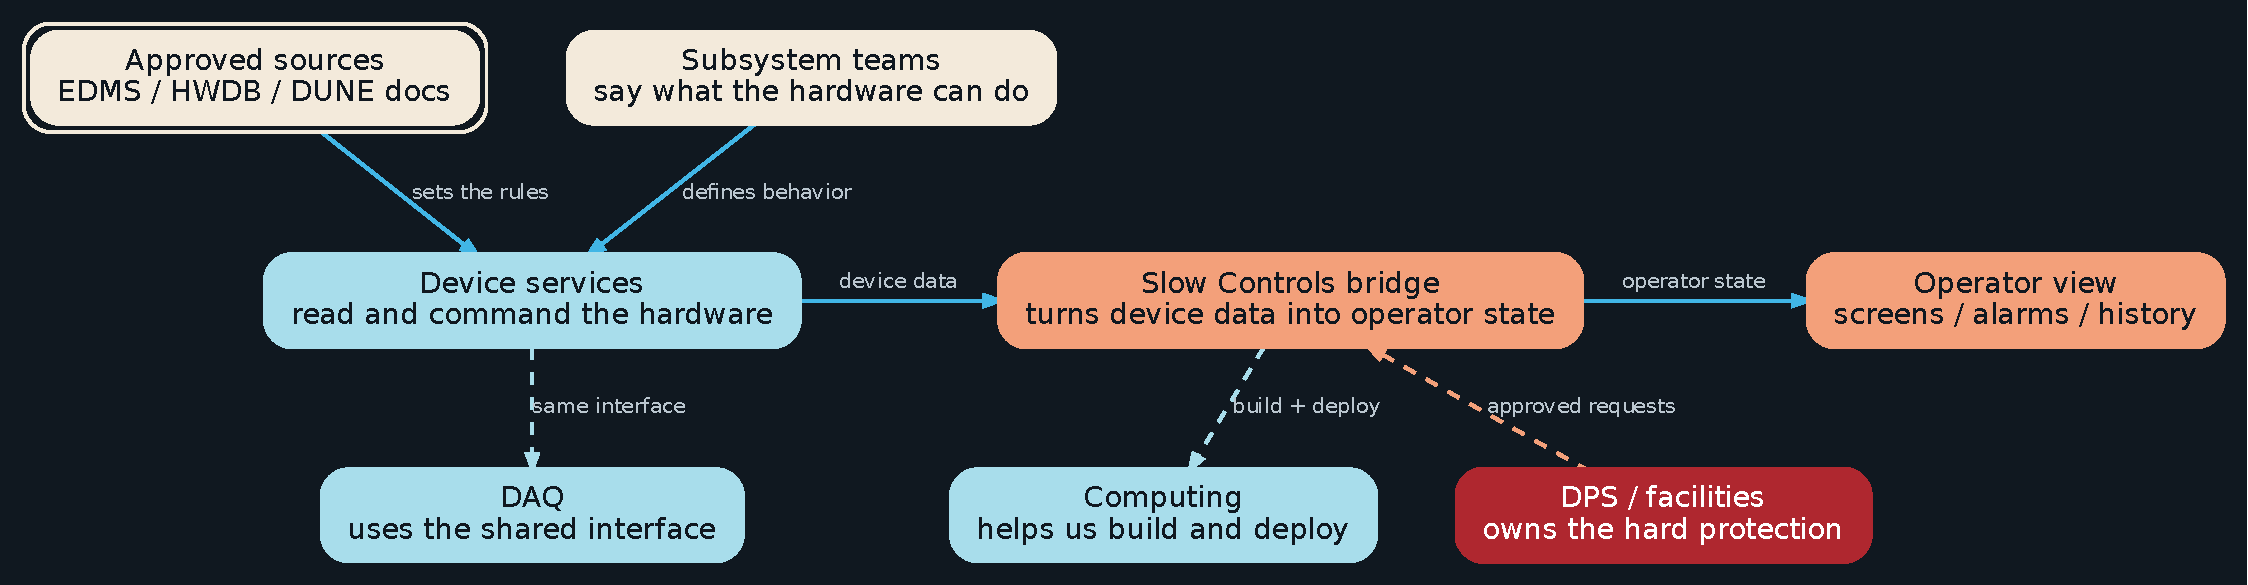
\includegraphics[width=0.96\textwidth,height=0.62\textheight,keepaspectratio]{diagrams/system-context.pdf}

  \smallskip
  \DuneDiagramCaption{The subsystem defines what the device can do. Slow Controls turns that into a reliable operator view. DPS still owns protection.}
\end{frame}

\begin{frame}{DAPHNE and WIB need one shared language}
  \centering
  \begin{tikzpicture}
    \node[sc paper,minimum width=5.2cm] (contract) at (0,1.35)
      {Shared, versioned interface\\states / commands / errors / freshness};
    \node[sc sky] (daq) at (-4.15,-0.85)
      {DAQ client\\run-control meaning};
    \node[sc coral] (bridge) at (0,-0.85)
      {SC bridge\\OPC-UA / quality\\alarms / history};
    \node[sc sky] (emulator) at (4.15,-0.85)
      {Emulator\\nominal / stale\\fault / recovery};
    \draw[sc arrow] (contract) -- (daq);
    \draw[sc warm arrow] (contract) -- (bridge);
    \draw[sc arrow] (contract) -- (emulator);
  \end{tikzpicture}

  \smallskip
  \DuneDiagramCaption{DAQ, Slow Controls, and the emulator should all read the same interface—no private translations.}
  \smallskip
  \DuneColorBlock{coral}{BEFORE WE RELEASE}{All three must agree}
    {The DAQ client, SC bridge, and emulator must prove that they understand the same version.}
\end{frame}

\begin{frame}{Rack software starts with what is really installed}
  \begin{columns}[T,onlytextwidth]
    \begin{column}{0.35\textwidth}
      \DuneBigStatement{FOLLOW THE FACTS}
        {The operator view starts with real rack and outlet names.}
        {Slow Controls can use those facts without taking ownership of the electrical system or its protection.}
    \end{column}
    \begin{column}{0.61\textwidth}
      \DuneCompactColorBlock{paper}{01 · INSTALLATION}{Tell us what is there}
        {Installation owners provide the rack, outlet, cable, and host mappings.}
      \vspace{0.25mm}
      \DuneCompactColorBlock{coral}{02 · SLOW CONTROLS}{Turn facts into a useful view}
        {The bridge adds data quality, alarms, command checks, and history.}
      \vspace{0.25mm}
      \DuneCompactColorBlock{sky}{03 · COMPUTING}{Help us run it reliably}
        {Computing reviews the hosts, network, build pipeline, artifacts, and deployment.}
    \end{column}
  \end{columns}
\end{frame}

\begin{frame}{Seeing a problem is not the same as stopping it}
  \begin{columns}[T,onlytextwidth]
    \begin{column}{0.48\textwidth}
      \DuneFixedColorBlock{sky}{3.35cm}{SLOW CONTROLS CAN}
        {Show and request}
        {\textbf{Make the situation visible}\par
         Show protection state, alarms, trends, and diagnostics.\par\medskip
         \textbf{Ask for an allowed action}\par
         Use an approved path with clear permissions and clear failure behavior.}
    \end{column}
    \begin{column}{0.48\textwidth}
      \DuneFixedColorBlock{coral}{3.35cm}{DPS / FACILITIES MUST}
        {Protect and authorize}
        {\textbf{Keep the hard protection independent}\par
         Interlocks must still work when ordinary software fails.\par\medskip
         \textbf{Approve any change to that line}\par
         Only the protection owner can change who carries this responsibility.}
    \end{column}
  \end{columns}

  \smallskip
  \DuneCompactColorBlock{danger}{THE HARD RULE}{The screen is not the safety system}
    {Unless the protection owner explicitly approves it, an HMI, bridge, or ordinary service is only a monitor—not an interlock.}
\end{frame}

\begin{frame}{For detector electronics, SC owns the bridge—not the device}
  \small
  \renewcommand{\arraystretch}{1.20}
  \begin{tabularx}{\textwidth}{@{}p{0.18\textwidth} p{0.39\textwidth} X@{}}
    \toprule
    System & Slow Controls is responsible for & We work with \\
    \midrule
    PDS / DAPHNE &
    \OwnerCell{The bridge and operator view}{OPC-UA mapping, data quality, alarms, and history.} &
    \OwnerCell{PDS and DAQ}{Board behavior, the shared interface, and DAQ compatibility.} \\
    \addlinespace
    TPC / BDE / WIB &
    \OwnerCell{The BDE/WIB bridge}{Readiness, operator commands, and bridge behavior.} &
    \OwnerCell{TPC/BDE and DAQ}{WIB limits and run-control integration.} \\
    \addlinespace
    Timing / TDE &
    \OwnerCell{The operator view}{State, quality, commands, alarms, and history.} &
    \OwnerCell{Timing and DAQ}{Timing behavior and data-taking limits.} \\
    \bottomrule
  \end{tabularx}
\end{frame}

\begin{frame}{For services, SC owns the view—not the infrastructure}
  \small
  \renewcommand{\arraystretch}{1.20}
  \begin{tabularx}{\textwidth}{@{}p{0.18\textwidth} p{0.39\textwidth} X@{}}
    \toprule
    System & Slow Controls is responsible for & We work with \\
    \midrule
    PDU / rack services &
    \OwnerCell{The monitoring bridge}{SNMP/IPMI mapping, stale-data rules, and alarms.} &
    \OwnerCell{Electrical, rack, and Computing}{Installed facts, hosts, network, and deployment.} \\
    \addlinespace
    HVS / calibration &
    \OwnerCell{The operator view}{Methods, readback quality, alarms, and history.} &
    \OwnerCell{Subsystem and safety owners}{Safe ranges, permissions, and approved modes.} \\
    \addlinespace
    DPS / facilities &
    \OwnerCell{Visibility}{Display, archive, alarms, and documented requests.} &
    \OwnerCell{DPS / facilities}{The protection logic and hard interlocks.} \\
    \bottomrule
  \end{tabularx}
\end{frame}

\DuneSectionPage{NOW MAP IT TO GIT}{Let the repository structure tell the same story}
  {Someone opening the code should be able to see where the facts, interfaces, bridge, operator view, and tests belong.}

\begin{frame}{The Git structure should match the way we work}
  \centering
  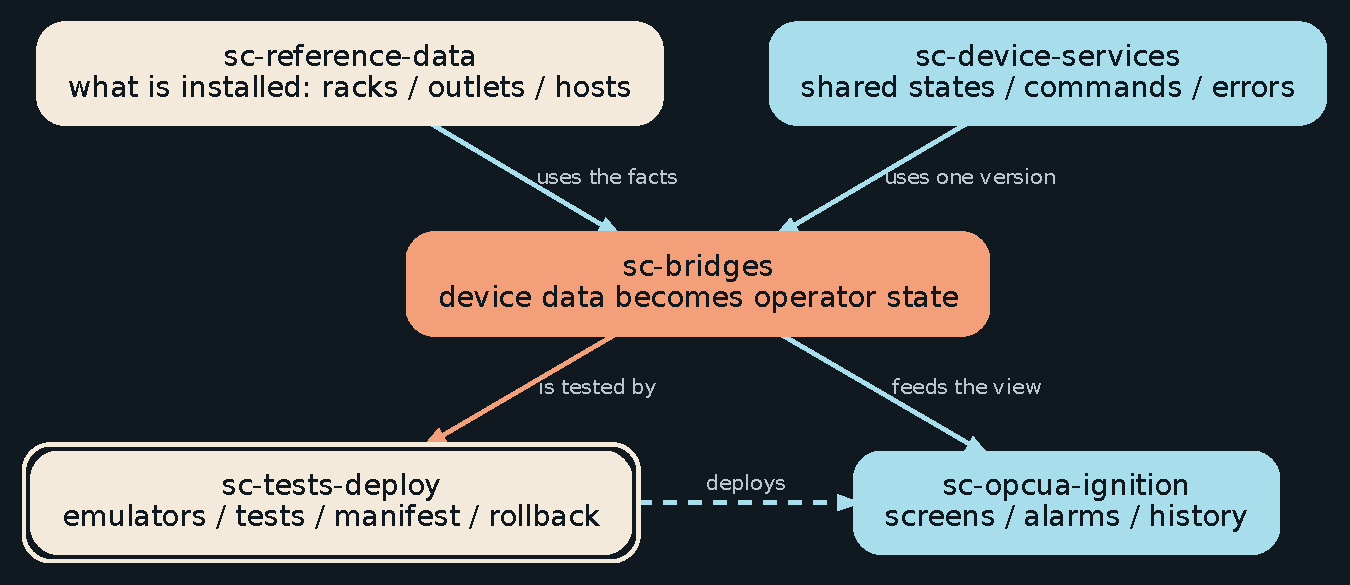
\includegraphics[width=0.94\textwidth,height=0.64\textheight,keepaspectratio]{diagrams/repository-architecture.pdf}

  \smallskip
  \DuneDiagramCaption{The installed facts and shared interface feed the SC bridge. The operator view and release proof stay visible as separate jobs.}
\end{frame}

\begin{frame}{A reviewer should find four things in every repository}
  \begin{columns}[T,onlytextwidth]
    \begin{column}{0.235\textwidth}
      \DuneNumberBlock{paper}{01}{The source}
        {Link the EDMS, HWDB, DUNE, or GitHub material that the code follows.}
    \end{column}
    \begin{column}{0.235\textwidth}
      \DuneNumberBlock{sky}{02}{The people}
        {Name the hardware, SC, DAQ, safety, and deployment reviewers who matter here.}
    \end{column}
    \begin{column}{0.235\textwidth}
      \DuneNumberBlock{sky}{03}{The interface}
        {Version the shared language. Say who uses it and what happens when it fails.}
    \end{column}
    \begin{column}{0.235\textwidth}
      \DuneNumberBlock{coral}{04}{The proof}
        {Include tests, compatibility results, a manifest, and a short rollback plan.}
    \end{column}
  \end{columns}

  \medskip
  {\centering\color{DuneTextMuted}\large
    The README explains the promise; the release tag shows we kept it.\par}
\end{frame}

\begin{frame}{Start small and prove the whole path}
  \framesubtitle{Use DAPHNE or WIB; make one shared interface work three ways}
  \begin{columns}[T,onlytextwidth]
    \begin{column}{0.31\textwidth}
      \vspace{10mm}
      \DuneNumberBlock{paper}{01}{Write the shared language}
        {Define the states, commands, errors, data age, and compatibility rules.}
    \end{column}
    \begin{column}{0.31\textwidth}
      \vspace{5mm}
      \DuneNumberBlock{sky}{02}{Use it in DAQ and SC}
        {One DAQ client and one Slow Controls bridge use exactly the same version.}
    \end{column}
    \begin{column}{0.31\textwidth}
      \DuneNumberBlock{coral}{03}{Test the bad days too}
        {An emulator checks normal operation, stale data, faults, and recovery.}
    \end{column}
  \end{columns}

  \medskip
  {\color{DuneCoral}\rule{\textwidth}{1.2pt}\par}
  {\footnotesize\bfseries Do not argue about names first. A working example will show us where the clean split belongs.}
\end{frame}

\begin{frame}{What we need to decide on Thursday}
  \begin{columns}[T,onlytextwidth]
    \begin{column}{0.35\textwidth}
      \DuneFixedColorBlock{coral}{3.55cm}{WHAT I AM ASKING FOR}
        {Leave with clear owners and a first test}
        {Choose the responsibility and review rules now. Let repository names follow from them.}
    \end{column}
    \begin{column}{0.61\textwidth}
      \begin{enumerate}
        \DuneTightList
        \item Agree to assign responsibility before repositories.
        \item Confirm that SC owns the DAPHNE/WIB operator bridges.
        \item Choose where these repositories will live on GitHub.
        \item Name the reviewers and choose DAPHNE or WIB for the first working example.
      \end{enumerate}
    \end{column}
  \end{columns}

  \smallskip
  \DuneCompactColorBlock{paper}{WE ARE DONE WHEN}{One tagged release proves the idea}
    {One shared interface works in a DAQ client, an SC bridge, and an emulator—with named reviewers.}
\end{frame}

\end{document}
